\documentclass[12pt]{article}
\usepackage[T1]{fontenc}
\usepackage[polish]{babel}
\usepackage[utf8]{inputenc}
\usepackage{graphicx}
\usepackage{float}



%opening
\title{Dokumentacja aplikacji InstaCar}
\author{Sebastian Górski\\ Jakub Grzymisławski\\ Łukasz Szenkiel}
\date{\today}

\begin{document}

\maketitle

\newpage
\tableofcontents

\newpage
\section*{Opis}
\addcontentsline{toc}{section}{Opis}
	Dokumentacja dotyczy aplikacji \textit{InstaCar}, służącej do rezerwacji samochodów na wynajem. Aplikacja umożliwia użytkownikom przeglądanie dostępnych pojazdów, dokonywanie rezerwacji w wybranym terminie oraz zarządzanie swoimi rezerwacjami. Dokument zawiera szczegółowy opis funkcjonalności systemu, instrukcję użytkowania, wymagania techniczne oraz informacje przeznaczone dla administratorów i deweloperów.

\newpage
\section{Architektura systemu}
W tej sekcji przedstawiono opis architektury systemu \textit{Instacar}.
\subsection{Diagram klas}
Diagram klas przedstawia strukturę aplikacji \textit{InstaCar} w ujęciu obiektowym, wraz z zależnościami między klasami.

\begin{figure}[H]
	\centering
	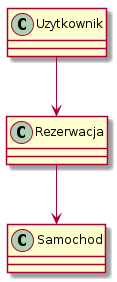
\includegraphics[width=0.3\linewidth, height=0.5\textheight]{diagramKlas}
	\caption{Diagram klas}
	\label{fig:diagramklas.png}
\end{figure}


\subsection{Diagram czynności}
Diagram czynności ilustruje przebieg głównych procesów w aplikacji, takich jak rezerwacja pojazdu czy logowanie użytkownika.

\subsection{Diagram przypadków użycia}
Diagram przypadków użycia ukazuje interakcje użytkowników z systemem, identyfikując główne funkcje dostępne w aplikacji.

\subsection{Implementacja kodu}
Ta część zawiera informacje dotyczące technologii użytych przy implementacji oraz struktury katalogów i plików w projekcie.

\section{Interfejs użytkownika}
\section{Dokumentacja użytkowa}
\section{Bibliografia}

\end{document}
